\documentclass{beamer}
\usepackage[subpreambles=true]{standalone}
\usepackage{tabulary}

%****************************************************************
% Some settings
%****************************************************************
\usecolortheme{beaver}
\usefonttheme{default}
\usetheme{CambridgeUS}

%\graphicspath{{figures/}}

\setbeamertemplate{navigation symbols}{}

%****************************************************************
% Define color
%****************************************************************
\definecolor{MITred}{RGB}{163,31,52}
\definecolor{MITgray}{RGB}{138,139,140}
\definecolor{MITlightgray}{RGB}{194,192,191}

%****************************************************************
% Modify footline & headline
%****************************************************************
%gets rid of bottom navigation bars
\setbeamertemplate{footline}[frame number]{}

%gets rid of header
\setbeamertemplate{headline}{}

%****************************************************************
% Modify title
%****************************************************************
\setbeamertemplate{title page}[default][colsep=-4bp,rounded=true]

%****************************************************************
% Modify table of contents
%****************************************************************
\setbeamertemplate{section in toc}{{\color{MITred}%
  \MakeUppercase{\romannumeral \inserttocsectionnumber}.}%
~\inserttocsection}
\setbeamertemplate{subsection in toc}{\hspace{1.2em}{\color{MITred}%
{\tiny $\blacksquare$}}~\inserttocsubsection \par}
\setbeamertemplate{subsubsection in toc}{\hspace{2.4em}%
{\color{MITred}{\tiny $\square$}}~\inserttocsubsection \par}

%****************************************************************
% Modify frame
%****************************************************************
\setbeamercolor{frametitle}{fg=MITred}
\setbeamertemplate{blocks}[rounded][shadow=false]
\setbeamercolor{block title}{fg=MITred}

%****************************************************************
% Modify numerate & itemize bullet
%****************************************************************
\setbeamercolor{enumerate item}{fg=MITred}
\setbeamercolor{enumerate subitem}{fg=MITred}
\setbeamercolor{enumerate subsubitem}{fg=MITred}
\setbeamertemplate{enumerate items}[default]

\setbeamercolor{itemize item}{fg=MITred}
\setbeamercolor{itemize subitem}{fg=MITred}
\setbeamercolor{itemize subsubitem}{fg=MITred}
\setbeamertemplate{itemize item}[triangle]
\setbeamertemplate{itemize subitem}{$\triangleright$}
\setbeamertemplate{itemize subsubitem}{$\bullet$}

%****************************************************************
% Some definitions
%****************************************************************
\providecommand{\figurepath}{figures}

%****************************************************************
% Title
%****************************************************************
\title[Title]
{hIPPYlib-MUQ: Scalable Markov chain Monte Carlo sampling methods for
large-scale Bayesian inverse problems governed by PDEs}
%\subtitle{Short title}
\author[Kim et al.]{Ki-Tae Kim\inst{1}\\ \vspace{0.5cm} Noemi Petra\inst{1}
  \and Umberto Villa\inst{2} \and Matthew Parno\inst{3} \\ \and Youssef
Marzouk\inst{4} \and Omar Ghattas\inst{5}}
\institute[]
{\inst{1}University of California, Merced \and \inst{2}Washington University in
St. Louis \and \inst{3}The United States Army Corps of Engineers \and \inst{4}
Massachusetts Institute of Technology \and \inst{5} The University of Texas at
Austin}

\date[\today]{\today}

%****************************************************************
% Begin document
%****************************************************************
\begin{document}

\makeatletter
\def\beamer@andinst{\\[0.2em]}
\makeatother

\begin{frame}[noframenumbering,plain]
  \titlepage

  \vspace{-0.4cm}
  {\scriptsize The FEniCS 2021 conference \hfill NSF grants ACI-1550487,
  ACI-1550547, ACI-1550593}
\end{frame}

\begin{frame}[c]
  \frametitle{Inverse problems governed by PDEs}
  \begin{center}
    \includestandalone[width=\textwidth]{tikz/inverse_problems}
  \end{center}

  \begin{itemize}
    \item [] \scriptsize{Details in: T. Isaac, N. Petra, G. Stadler, and
                 O. Ghattas, Journal of Computational Physics (2015)}
  \end{itemize}
\end{frame}

\begin{frame}[c]
  \frametitle{Bayesian inference framework}

  \begin{center}
    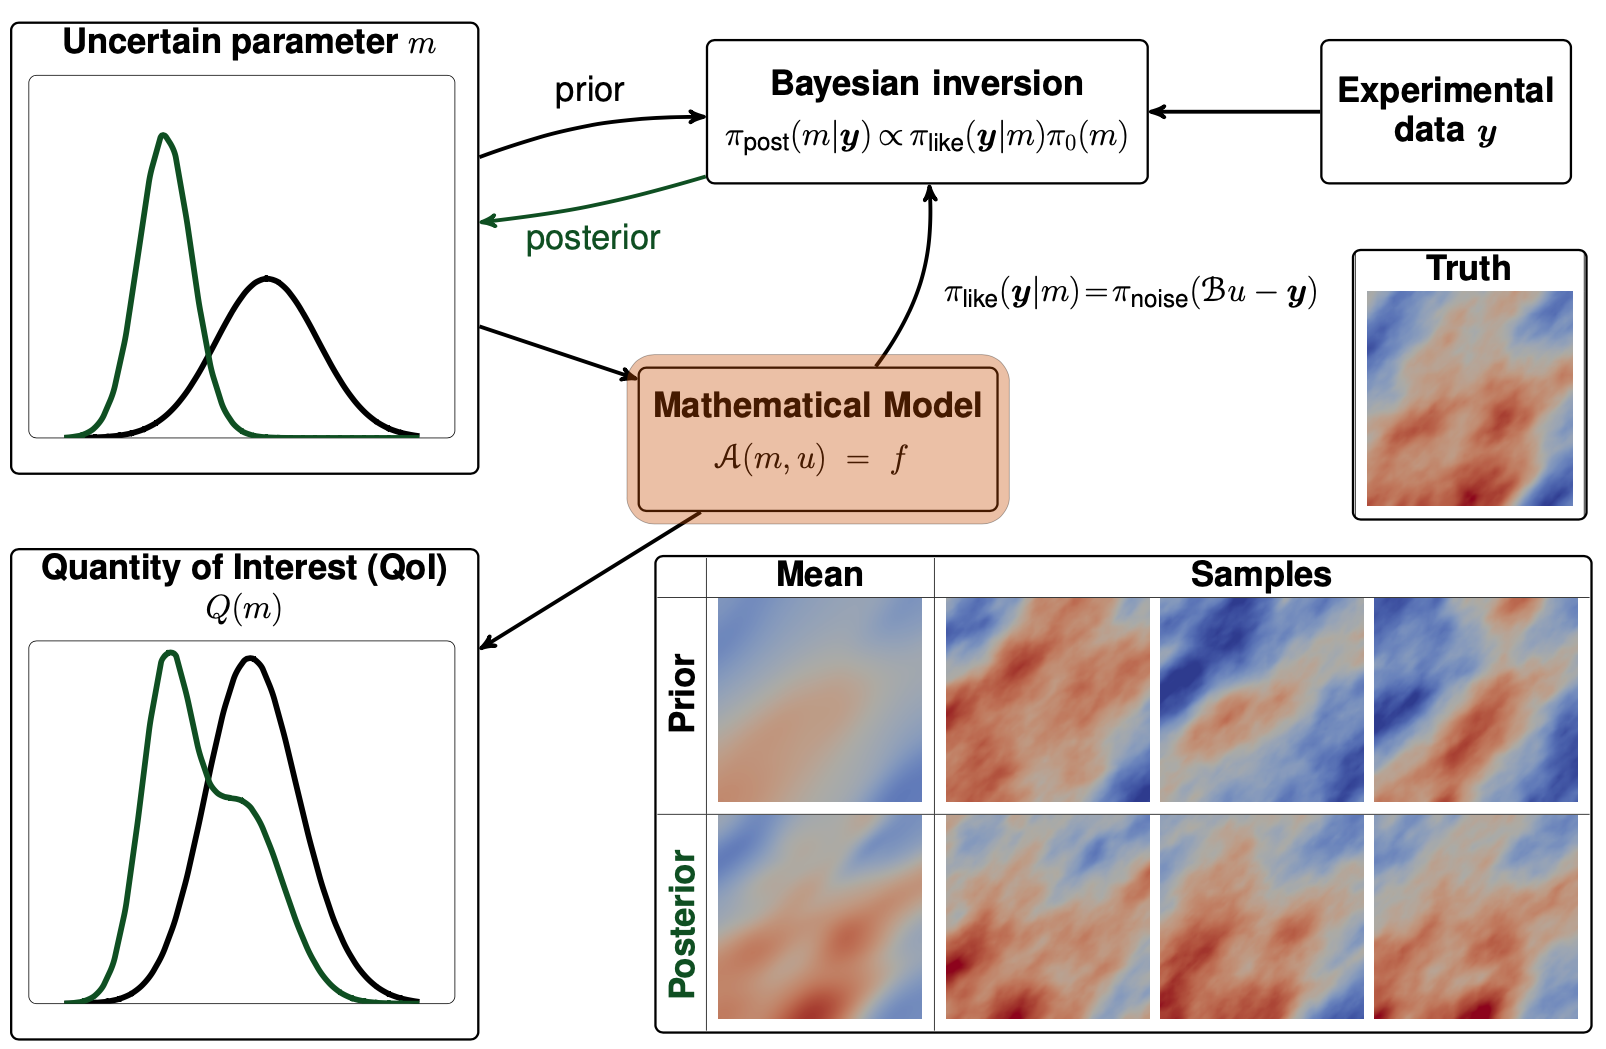
\includegraphics[width=\textwidth]{./figures/bayesian_framework.png}
  \end{center}
\end{frame}

\begin{frame}[c]
  \frametitle{Motivation and challenges}

  \begin{alertblock}{Bayesian framework}
    \begin{itemize}
      \item {\bf Combines data with complex models to make better predictions}
        \vspace{-0.5cm}
        \begin{itemize}
          \item Application area: geosciences, mechanics,
            materials, aerospace, electronics, biological sciences,
            chemical systems, medicine, ...
        \end{itemize}
      \item {\bf Quantifies the uncertainty} in the solution of inverse
        problems
    \end{itemize}
  \end{alertblock}

  \begin{alertblock}{Markov Chain Monte Carlo (MCMC)}
    \begin{itemize}
      \item Common method for solving Bayesian inverse problems governed by
        PDEs
      \item {\bf Prohibitive for large and complex problems} $\rightarrow$ Solution
          via conventional MCMC is intractable
    \end{itemize}
  \end{alertblock}

  \begin{alertblock}{Goal}
    \begin{itemize}
      \item Develop scalable open-source software to overcome the
        prohibitive nature of Bayesian inversion
      \item Make advanced inversion capabilities available to a broader
        scientific community and accelerate scientific discovery
    \end{itemize}
  \end{alertblock}

\end{frame}

\begin{frame}[c]
  \frametitle{hIPPYlib-MUQ integration}
   \begin{center}
    \includestandalone[width=\textwidth]{tikz/integration_diagram}
  \end{center}

  \begin{itemize}
    \item hIPPYlib: aimed at solving deterministic and linearized Bayesian
      inverse problems governed by PDEs
    \item MUQ: aimed at solving uncertainty quantification problems
  \end{itemize}
\end{frame}

\begin{frame}[c]
  \frametitle{Key feature: Hessian informed MCMC}

  \begin{tabulary}{\linewidth}{CC}
    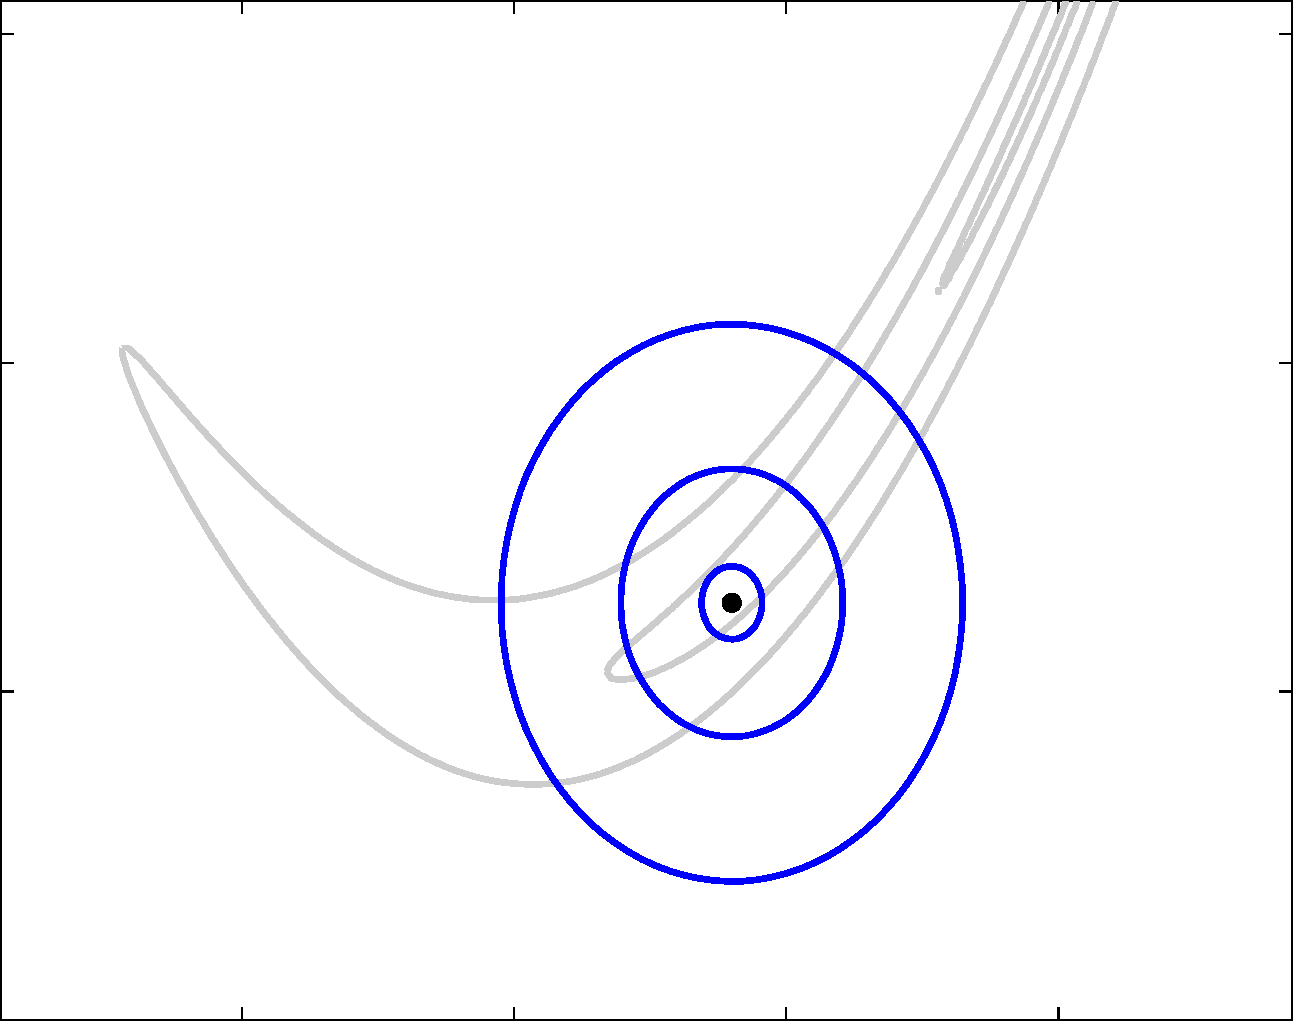
\includegraphics[width=0.45\textwidth]{./figures/mcmcprop_iso.pdf}
    &
    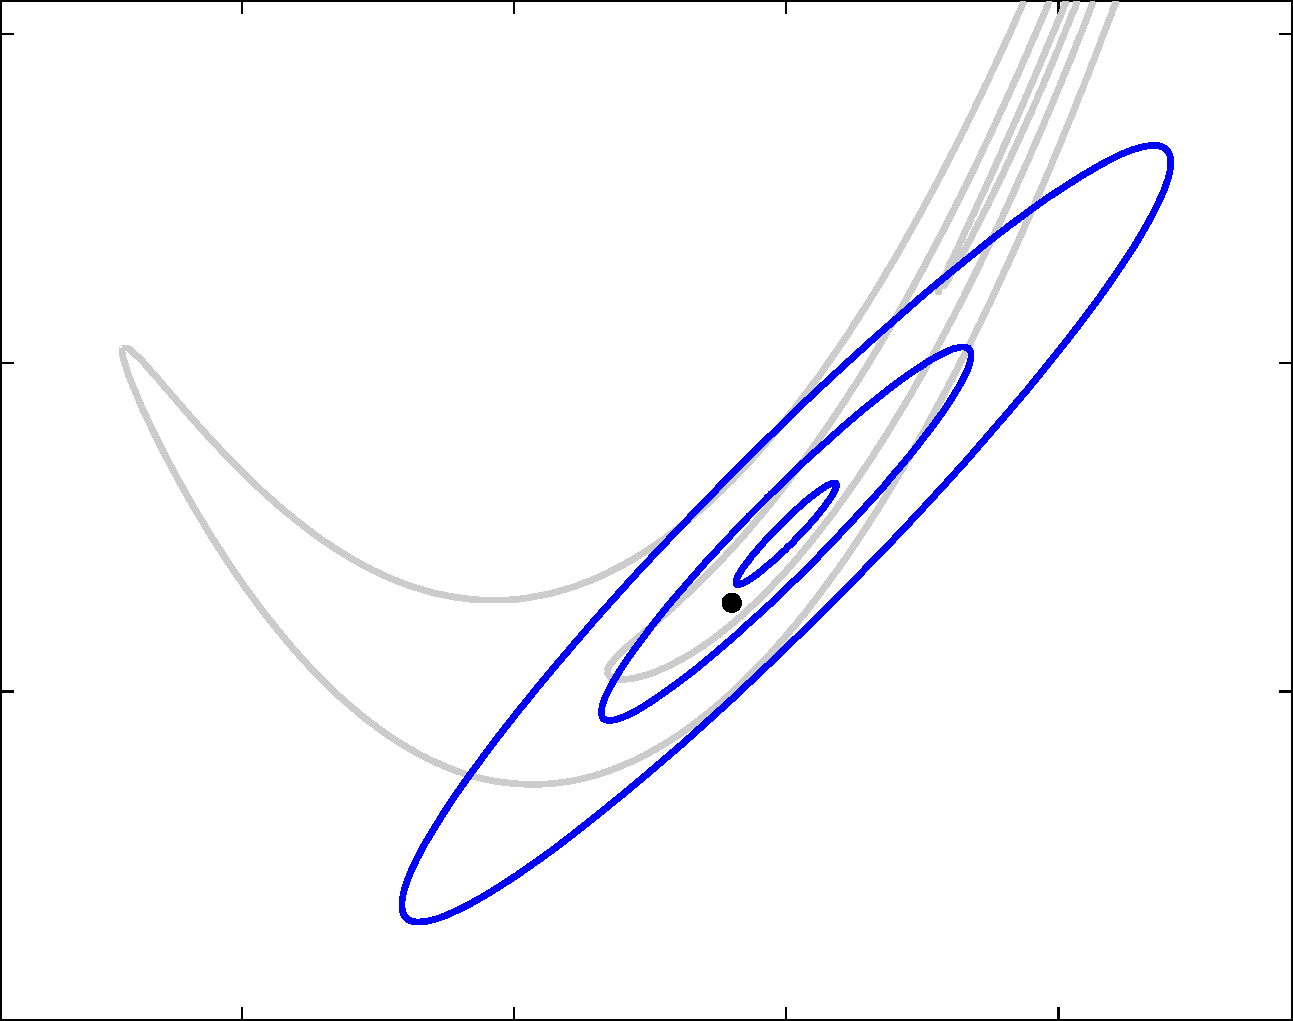
\includegraphics[width=0.45\textwidth]{./figures/mcmcprop_curvature.pdf}
    \\
    Typical isotropic MCMC proposal
    &
    Curvature (Hessian) aware MCMC proposal
  \end{tabulary}

  \vspace{0.5cm}

  hIPPYlib-MUQ enables Hessian informed MCMC that
  \begin{itemize}
    \item exploits the curvature (Hessian) of the posterior $\rightarrow$
      significant improvement of sampling performance
    \item uses low rank approximation of the Hessian $\rightarrow$ efficient
      Hessian operation
  \end{itemize}

\end{frame}

\begin{frame}[c]
  \frametitle{Example -- subsurface flow}

  \begin{tabular}{cc}
    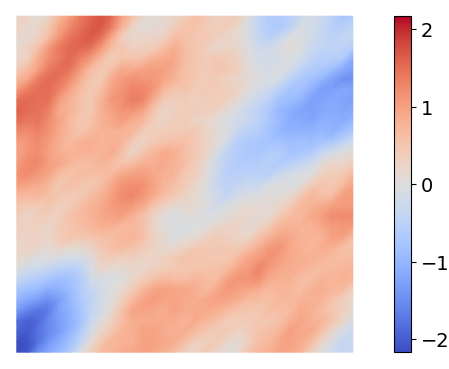
\includegraphics[width=0.45\textwidth]{./figures/ex1_true_parameter.png}
    &
    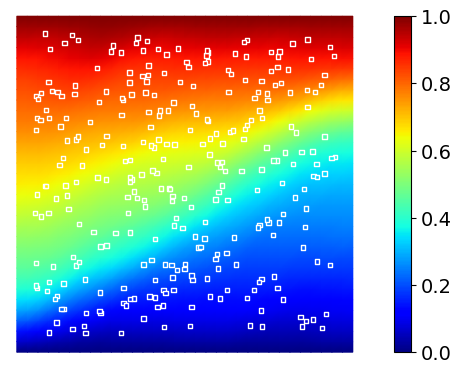
\includegraphics[width=0.45\textwidth]{./figures/ex1_true_state_observation.png}
    \\
    True parameter $m_{\text{true}}$
    &
    Obervations $y$
  \end{tabular}

  \vspace{0.3cm}

  Bayes' theorem:
  \[
    \pi_{\text{post}} (m|y) \propto \pi_{\text{like}} (y|m)
    \pi_{0} (m)
  \]

  \begin{itemize}
    \item Forward model: $\nabla \cdot (e^m \nabla u) = 0$ ($u=1$ on top,
      $u=0$ on bottom, and no flux on left and right)
    \item Gaussian prior with zero mean and Laplacian-like covariance operator
  \end{itemize}
\end{frame}

\begin{frame}[c]
  \frametitle{MAP point and Laplace approximation of the posterior}

  \begin{center}
    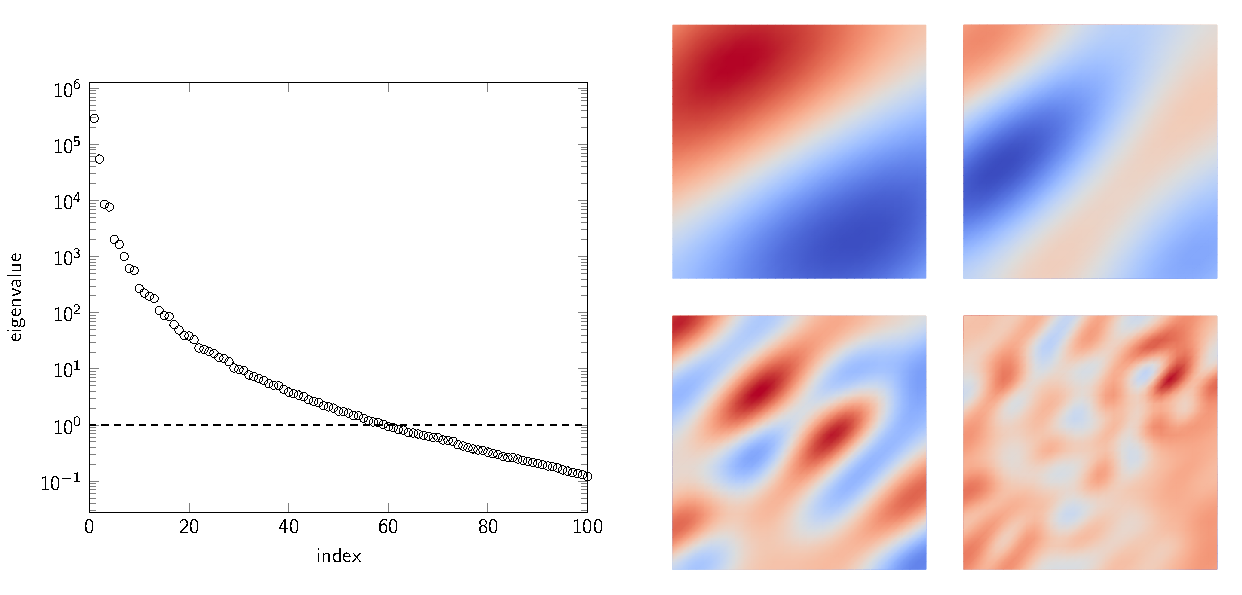
\includegraphics[width=0.7\textwidth]{./figures/ex1_misfit_eig.pdf}

    {\tiny Eigenvalues and eigenvectors (1st, 4th, 16th, and 64th largest) of the
    Hessian (the number of data $= 300$)}
    % 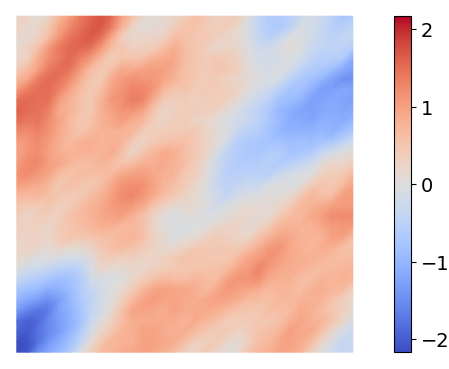
\includegraphics[width=0.2\textwidth]{./figures/ex1_true_parameter.png}
    % 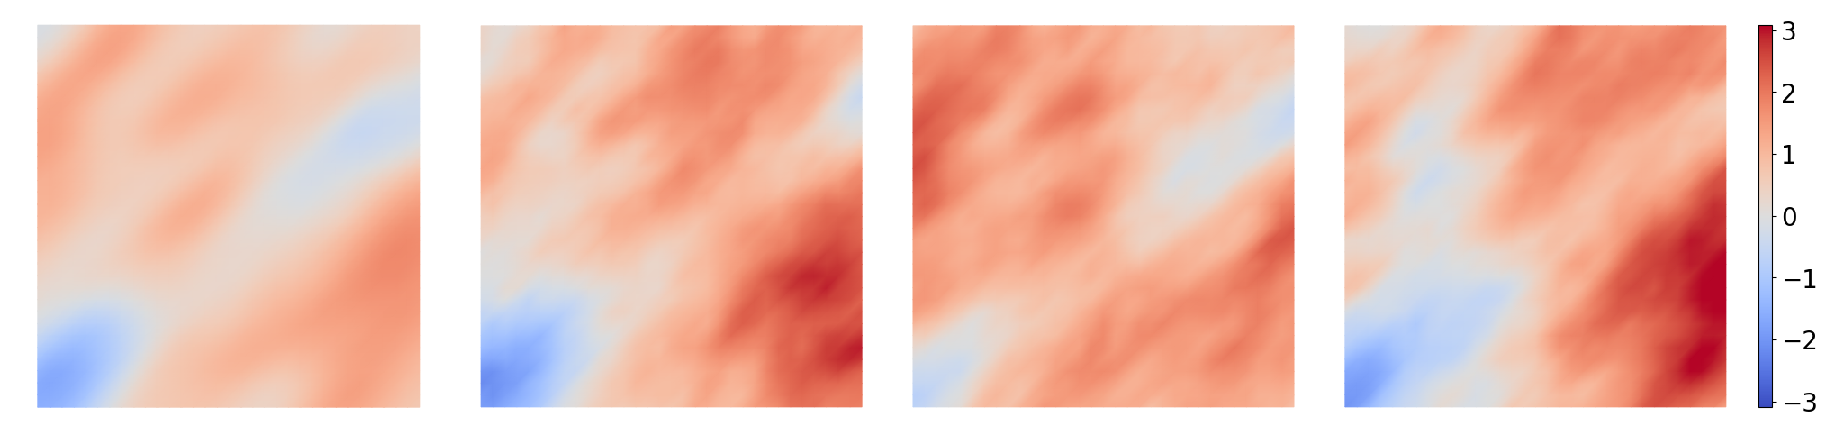
\includegraphics[width=0.7\textwidth]{./figures/ex1_la_samples.pdf}
    %
    % {\footnotesize True, The MAP point (leftmost) and three samples from the Laplace approximation}
  \end{center}

  \begin{tabulary}{\linewidth}{CC}
    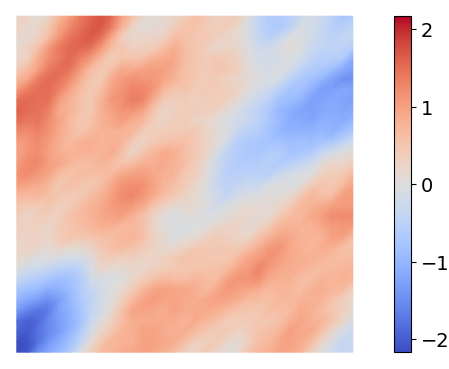
\includegraphics[height=0.24\textheight]{./figures/ex1_true_parameter.png}
    &
    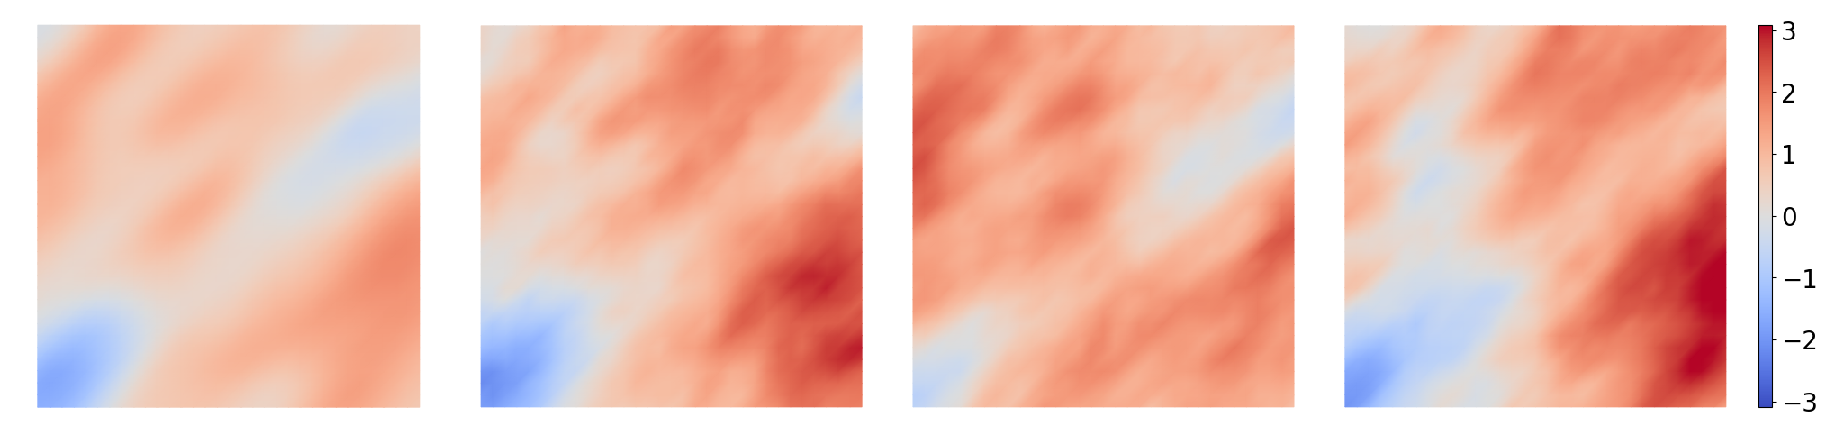
\includegraphics[height=0.24\textheight]{./figures/ex1_la_samples.pdf}
    \\
    {\tiny True}
    &
    {\tiny The MAP point (leftmost) and three samples from the Laplace
    approximation}
  \end{tabulary}

  \vspace{0.1cm}

  \begin{itemize}
    \item Laplace approximation: $\pi_{\text{post}} \approx
      \hat{\pi}_{\text{post}} \sim \mathcal{N} (m_{\text{MAP}},
      \mathcal{H}^{-1} (m_{\text{MAP}}))$
  \end{itemize}
\end{frame}

\begin{frame}[c]
  \frametitle{MCMC to explore the posterior}

  \begin{tabulary}{\linewidth}{CC}
    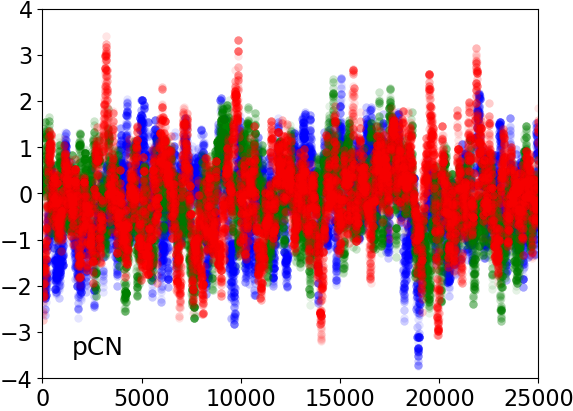
\includegraphics[width=0.45\textwidth]{./figures/ex1_LargeNoise_trace_pcn.png}
    &
    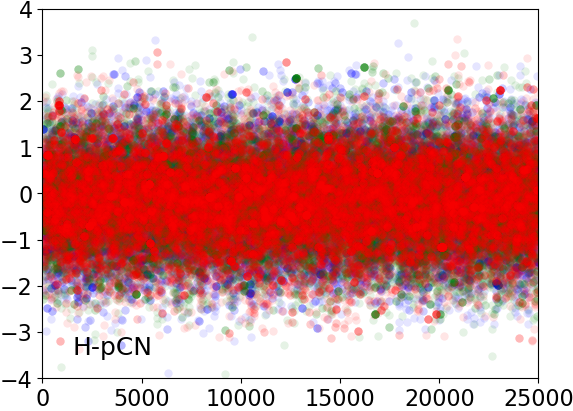
\includegraphics[width=0.45\textwidth]{./figures/ex1_LargeNoise_trace_hpcn.png}
    \\
    {\tiny using the prior as the MCMC proposal}
    &
    {\tiny using the Laplace approximation as the MCMC proposal}
  \end{tabulary}

  \begin{center}
    \begin{tabular}{cccc}
      Method & AR(\%) & MPSRF & ESS
      \\
      \hline
      pCN & 33 & 1.507 & 1,678
      \\
      H-pCN & 65 & 1.011 & 63,771
    \end{tabular}
  \end{center}

  \begin{itemize}
    \item 500,000 samples (25 independent chains)
    \item Significant improvement is achieved when the Hessian information (the
      Laplace approximation) is
      used
  \end{itemize}
\end{frame}

\begin{frame}[c]
  \frametitle{Comparison of various advanced MCMC methods}

  \begin{center}
    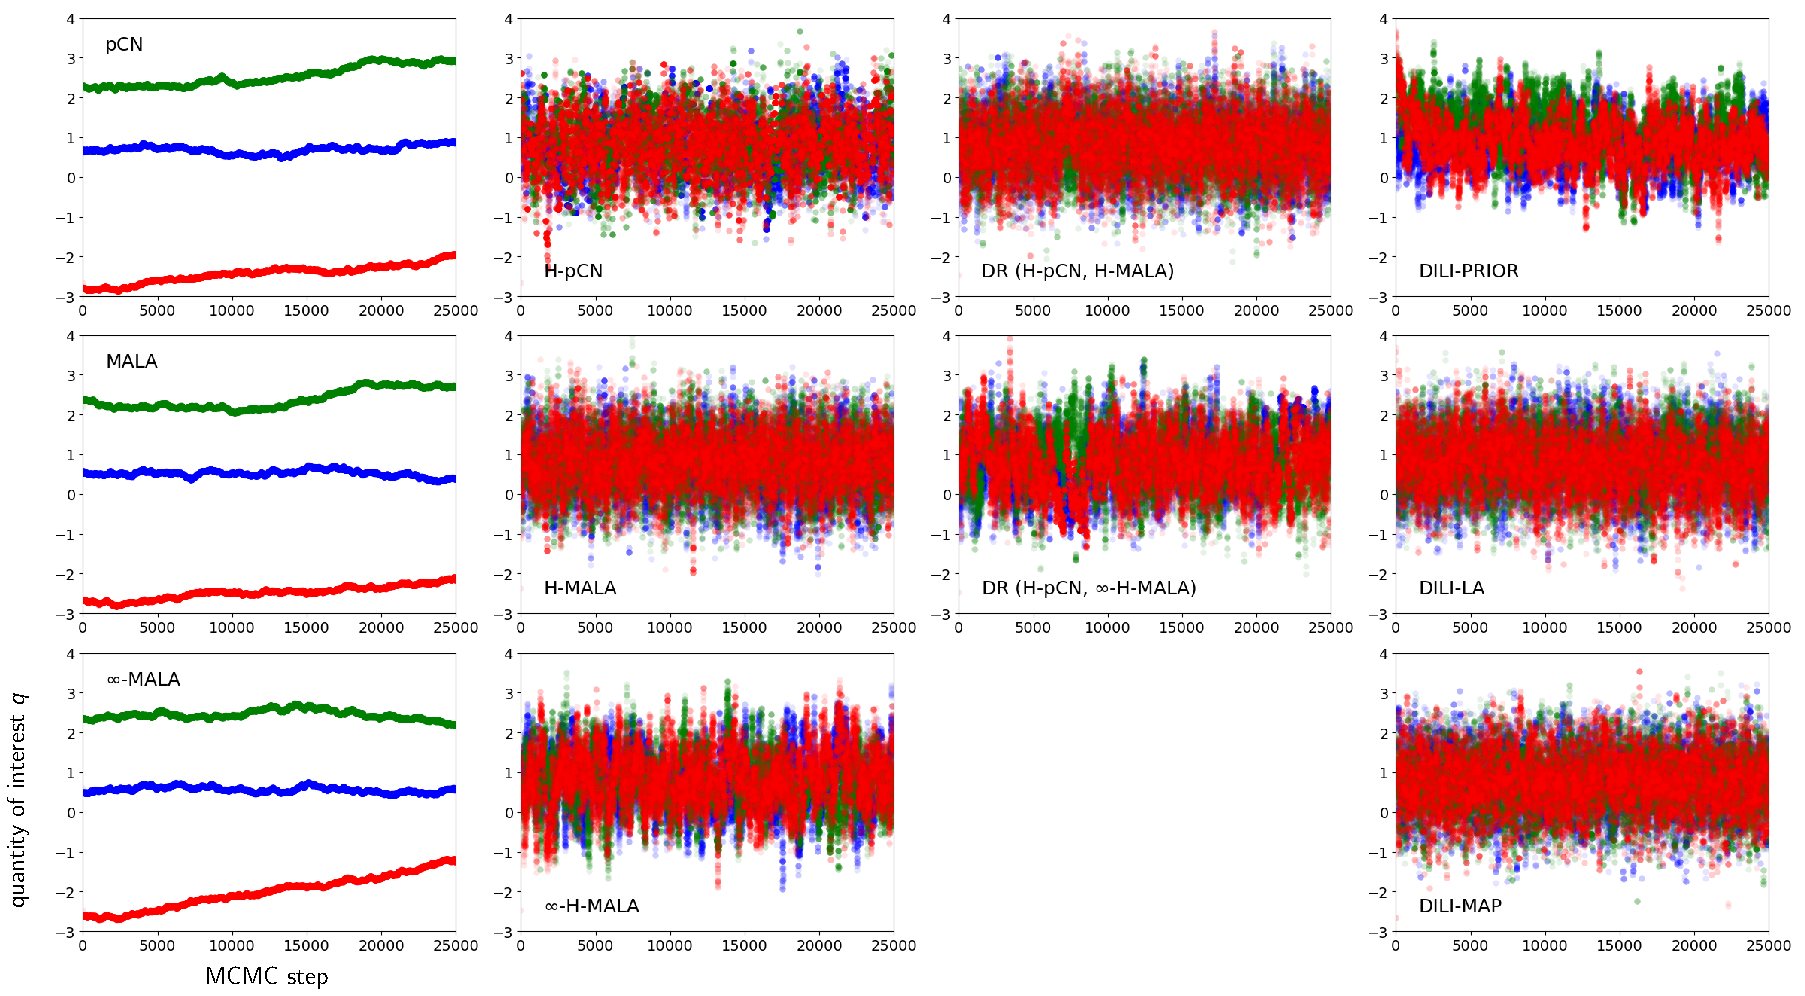
\includegraphics[width=\textwidth]{./figures/ex1_mcmc_trace.pdf}
  \end{center}

  \begin{itemize}
    \item Various advanced MCMC methods are available: Delayed rejections,
      Dimension independent likelihood informed, adaptive MCMC, ...
  \end{itemize}
\end{frame}

\begin{frame}[c]
  \frametitle{Summary}

  \begin{alertblock}{Bayesian framework}
    \begin{itemize}
      \item Provides a systematic approach for {\bf inferring predictive
          information from data and models with associated uncertainty}
      \item {\bf Prohibitive with conventional MCMC methods} for large and complex
        problems
    \end{itemize}
  \end{alertblock}

  \begin{alertblock}{Our contribution}
    \begin{itemize}
      \item Develop {\bf 'hIPPYlib-MUQ' that exploits problem structure} (curvature,
        low dimensionality) for
        \begin{itemize}
          \item Solving complex inverse problems governed by PDEs
          \item Quantifying associated uncertainty
        \end{itemize}
    \end{itemize}
  \end{alertblock}

  \begin{alertblock}{Software and paper}
    \begin{itemize}
      \item https://github.com/hippylib/hippylib2muq
      \item \scriptsize{K.T. Kim, N. Petra, U.  Villa, M. Parno, Y. Marzouk, and O. Ghattas,
        ACM Trans. Math. Software, in preparation}
    \end{itemize}
  \end{alertblock}

\end{frame}

\end{document}
